\def\mytitle{IDE ASSIGMNMENT}
\def\myauthor{NARENDRA MANIKANTA}
\def\contact{manikantakesana0@gmail.com}
\def\mymodule{Future Wireless Communications (FWC)}
\documentclass[journal,12pt,twocolumn]{IEEEtran}

\usepackage{setspace}
\usepackage{gensymb}
\usepackage{xcolor}
\usepackage{caption}
\usepackage[hyphens,spaces,obeyspaces]{url}
\usepackage[cmex10]{amsmath}
\usepackage{mathtools}
\usepackage{enumitem}
\usepackage{tikz}
\usetikzlibrary{automata, positioning}

\usepackage{enumitem}
\usepackage{circuitikz}
\usepackage{karnaugh-map}
\usepackage{tabularx}
\usepackage{tikz}
\singlespacing
\usepackage{amsthm}
\usepackage{mathrsfs}
\usepackage{txfonts}
\usepackage{stfloats}
\usepackage{cite}
\usepackage{cases}
\usepackage{subfig}
\usepackage{longtable}
\usepackage{multirow}
\twocolumn


\usepackage{graphicx}
\graphicspath{{./images/}}
\usepackage[colorlinks,linkcolor={black},citecolor={blue!80!black},urlcolor={blue!80!black}]{hyperref}
\usepackage[parfill]{parskip}
\usepackage{lmodern}
\usepackage{tikz}
\usepackage{circuitikz}
\usepackage{karnaugh-map}
\usepackage{pgf}
\usepackage[hyphenbreaks]{breakurl}

\usepackage{tabularx}
\usetikzlibrary{calc}

\renewcommand*\familydefault{\sfdefault}
\usepackage{watermark}
\usepackage{lipsum}
\usepackage{xcolor}
\usepackage{listings}
\usepackage{float}
\usepackage{titlesec}
\DeclareMathOperator*{\Res}{Res}
\renewcommand\thesection{\arabic{section}}
\renewcommand\thesubsection{\thesection.\arabic{subsection}}
\renewcommand\thesubsubsection{\thesubsection.\arabic{subsubsection}}

\renewcommand\thesectiondis{\arabic{section}}
\renewcommand\thesubsectiondis{\thesectiondis.\arabic{subsection}}
\renewcommand\thesubsubsectiondis{\thesubsectiondis.\arabic{subsubsection}}
\titlespacing{\subsection}{1pt}{\parskip}{3pt}
\titlespacing{\subsubsection}{0pt}{\parskip}{-\parskip}
\titlespacing{\paragraph}{0pt}{\parskip}{\parskip}
\newcommand{\figuremacro}[5]{
    \begin{figure}[#1]
        \centering
        \includegraphics[width=#5\columnwidth]{#2}
        \caption[#3]{\textbf{#3}#4}
        \label{fig:#2}
    \end{figure}
}

\lstset{
frame=single, 
breaklines=true,
columns=fullflexible
}

%\thiswatermark{\centering \put(400,-128.0){\includegraphics[scale=0.3]{logo}} }
\title{\mytitle}
\author{\myauthor\hspace{1em}\\\contact\\IITH\hspace{0.5em}-\hspace{0.6em}\mymodule}
\date{20-12-2022}
\def\inputGnumericTable{}                                 %%
\lstset{
%language=C,
frame=single, 
breaklines=true,
columns=fullflexible
}
 \begin{document}
%

\theoremstyle{definition}
\newtheorem{theorem}{Theorem}[section]
\newtheorem{problem}{Problem}
\newtheorem{proposition}{Proposition}[section]
\newtheorem{lemma}{Lemma}[section]
\newtheorem{corollary}[theorem]{Corollary}
\newtheorem{example}{Example}[section]
\newtheorem{definition}{Definition}[section]
%\newtheorem{algorithm}{Algorithm}[section]
%\newtheorem{cor}{Corollary}
\newcommand{\BEQA}{\begin{eqnarray}}
\newcommand{\EEQA}{\end{eqnarray}}
\newcommand{\define}{\stackrel{\triangle}{=}}
\bibliographystyle{IEEEtran}

\vspace{3cm}
\maketitle
\tableofcontents



\section{\textbf{Question}}
A sequence detector is designed to detect precisely 3 digital inputs, with overlapping sequence detectable. For the sequence $(1,0,1)$ and input data $(1,1,0,1,0,0,1,1,0,1,0,1,1,0)$ 
\begin{enumerate}
    \item 1,1,0,0,0,0,1,1,0,1,0,0
    \item 0,1,0,0,0,0,0,1,0,1,0,0
    \item 0,1,0,0,0,0,0,1,0,1,1,0
    \item 0,1,0,0,0,0,0,1,0,1,0,0
\end{enumerate}






  \section{\textbf{Answer}} 
The above question can be solved by using State diagram, Truth Table and karnaugh-map.\\
 
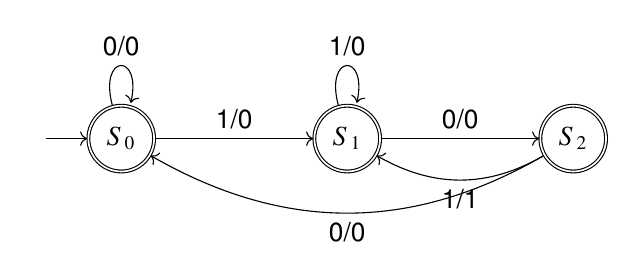
\begin{tikzpicture}[node distance=2cm, initial text={}]
  \node[state, initial, accepting] (S0) {$S_0$};
  \node[state, accepting, right=of S0] (S1) {$S_1$};
  \node[state, accepting, right=of S1] (S2) {$S_2$};
  
  \path[->] (S0) edge[above] node{1/0} (S1)
        (S0) edge[loop above] node{0/0} (S0)
        (S1) edge[above] node{0/0} (S2)
        (S1) edge[loop above] node{1/0} (S1)
        (S2) edge[below,bend left] node{1/1} (S1)
        (S2) edge[below,bend left] node{0/0} (S0);
\end{tikzpicture}
\subsection{\centering Truth Table}
\begin{tabularx}{0.45\textwidth}{
	| >{\centering\arraybackslash}X
	| >{\centering\arraybackslash}X
	| >{\centering\arraybackslash}X
	| >{\centering\arraybackslash}X
    | >{\centering\arraybackslash}X
    | >{\centering\arraybackslash}X
    | >{\centering\arraybackslash}X
	| >{\centering\arraybackslash}X|
	}\hline
	\textbf{$p$}&\textbf{$q$}&\textbf{$x$}&\textbf{$\bar p$}&\textbf{$\bar q$}&\textbf{$y$}&\textbf{$D1$}&\textbf{$D2$}\\
	\hline
	0&0&0&0&0&0&0&0\\
	\hline
	0&0&1&0&1&0&0&1\\
	\hline
    0&1&0&1&0&0&1&0\\
	\hline
	0&1&1&0&1&0&0&1\\
	\hline
	1&0&0&0&0&0&0&0\\
	\hline
	1&0&1&0&1&1&0&1\\
	\hline
	1&1&0&x&x&x&x&x\\
	\hline
	1&1&1&x&x&x&x&x\\
	\hline
\end{tabularx}
\begin{center} 
 Truth table for Boolean function
\end{center}
\subsection{\centering K-Map Implementation of $y$}
\resizebox{0.45\textwidth}{!}{%
	\begin{karnaugh-map}[4][2][1][$qx$][$p$]
		\maxterms{0,1,2,3,4}
		\minterms{5}
        \autoterms[X]
		\implicant{5}{7}
	\end{karnaugh-map}%
}
\begin{center}
Table. 1

herefore, the Boolean function is $y = px$.
\end{center}

\subsection{\centering K-Map Implementation of $D1$}
\resizebox{0.45\textwidth}{!}{%
	\begin{karnaugh-map}[4][2][1][$qx$][$p$]
		\maxterms{0,1,3,4,5}
		\minterms{2}
        \autoterms[X]
		\implicant{2}{6}
	\end{karnaugh-map}%
}
\begin{center}
Table. 2

Therefore, the Boolean function is $D1 = q\bar x$.
\end{center}

\subsection{\centering K-Map Implementation of $D2$}
\resizebox{0.45\textwidth}{!}{%
	\begin{karnaugh-map}[4][2][1][$qx$][$p$]
		\maxterms{0,2,4}
		\minterms{1,3,5}
        \autoterms[X]
		\implicant{1}{7}
	\end{karnaugh-map}%
}
\begin{center}
    Table. 3
    
    Therefore, the Boolean function is $D2 = x$.
\end{center}

	\section{\textbf{Components}}
	\begin{tabularx}{0.45\textwidth}{
			| >{\centering\arraybackslash}X
			| >{\centering\arraybackslash}X
			| >{\centering\arraybackslash}X|
			}
			\hline
			\textbf{Components}&\textbf{Values}&\textbf{Quantity}\\
			\hline
			Arduino & Uno & 1\\
			\hline
			Jumper Wires & M-M & 7\\
			\hline
			Breadboard & & 1\\
			\hline
   LED&&2\\
   \hline
   Resistor&220 ohms&2\\
   \hline
	\end{tabularx}
 
\section{\textbf{Implementation}}
\begin{tabularx}{0.45\textwidth}{
		| >{\centering\arraybackslash}X
		| >{\centering\arraybackslash}X
		| >{\centering\arraybackslash}X|}
\hline
	\textbf{Arduino PIN}&\textbf{INPUT}&\textbf{OUTPUT}\\
	\hline
	& 7&\\
	\hline
	8&&$LED$\\
	\hline
	3&&$LED$\\
	\hline

\end{tabularx}\\


\textbf{Procedure}
\begin{enumerate}[label={\arabic*}.]
	\item Connect the circuit as per the above table.
	\item Upload the code for arduino from the below link.
	\item verify the sequence manually fsm101\\
	\item note: it 8 pin is reference pin and 7 pin is input and 3 pin is over output

\begin{tabularx}{0.45\textwidth}{
		| >{\centering\arraybackslash}X|}
	\hline
	https://github.com/arduinojinarendra/fwc\_1\\may/blob/main/fwc/plaformio\_assignment.tex\\
	\hline

\end{tabularx}
	
\end{enumerate}


 \bibliographystyle{ieeetr}
\end{document}


